% THIS IS AN EXAMPLE DOCUMENT FOR VLDB 2012
% based on ACM SIGPROC-SP.TEX VERSION 2.7
% Modified by  Gerald Weber <gerald@cs.auckland.ac.nz>
% Removed the requirement to include *bbl file in here. (AhmetSacan, Sep2012)
% Fixed the equation on page 3 to prevent line overflow. (AhmetSacan, Sep2012)

%\documentclass[draft]{vldb}
\documentclass{vldb}
\usepackage{graphicx}
\usepackage{balance}  % for  \balance command ON LAST PAGE  (only there!)
\usepackage{fontspec}
\setmainfont[Ligatures={TeX}]{Times}
\usepackage{hyperref}
\graphicspath{{figures/}}

\hyphenation{metamarkets nelson}

\begin{document}

% ****************** TITLE ****************************************

\title{Druid: A Real-time Analytical Data Store}

% possible, but not really needed or used for PVLDB:
%\subtitle{[Extended Abstract]
%\titlenote{A full version of this paper is available as\textit{Author's Guide to Preparing ACM SIG Proceedings Using \LaTeX$2_\epsilon$\ and BibTeX} at \texttt{www.acm.org/eaddress.htm}}}

% ****************** AUTHORS **************************************

% You need the command \numberofauthors to handle the 'placement
% and alignment' of the authors beneath the title.
%
% For aesthetic reasons, we recommend 'three authors at a time'
% i.e. three 'name/affiliation blocks' be placed beneath the title.
%
% NOTE: You are NOT restricted in how many 'rows' of
% "name/affiliations" may appear. We just ask that you restrict
% the number of 'columns' to three.
%
% Because of the available 'opening page real-estate'
% we ask you to refrain from putting more than six authors
% (two rows with three columns) beneath the article title.
% More than six makes the first-page appear very cluttered indeed.
%
% Use the \alignauthor commands to handle the names
% and affiliations for an 'aesthetic maximum' of six authors.
% Add names, affiliations, addresses for
% the seventh etc. author(s) as the argument for the
% \additionalauthors command.
% These 'additional authors' will be output/set for you
% without further effort on your part as the last section in
% the body of your article BEFORE References or any Appendices.

\numberofauthors{7} %  in this sample file, there are a *total*
% of EIGHT authors. SIX appear on the 'first-page' (for formatting
% reasons) and the remaining two appear in the \additionalauthors section.

\author{
% You can go ahead and credit any number of authors here,
% e.g. one 'row of three' or two rows (consisting of one row of three
% and a second row of one, two or three).
%
% The command \alignauthor (no curly braces needed) should
% precede each author name, affiliation/snail-mail address and
% e-mail address. Additionally, tag each line of
% affiliation/address with \affaddr, and tag the
% e-mail address with \email.
%
% 1st. author
\alignauthor Fangjin Yang\\
\affaddr{Metamarkets Group, Inc.}\\
\affaddr{625 2nd Street, Suite 230}\\
\affaddr{San Francisco, CA, USA}\\
\email{fangjin@metamarkets.com}
\alignauthor Eric Tschetter\\
\affaddr{Metamarkets Group, Inc.}\\
\affaddr{625 2nd Street, Suite 230}\\
\affaddr{San Francisco, CA, USA}\\
\email{eric@metamarkets.com}
\alignauthor Gian Merlino\\
\affaddr{Metamarkets Group, Inc.}\\
\affaddr{625 2nd Street, Suite 230}\\
\affaddr{San Francisco, CA, USA}\\
\email{gian@metamarkets.com}
\and
\alignauthor Nelson Ray\\
\affaddr{Metamarkets Group, Inc.}\\
\affaddr{625 2nd Street, Suite 230}\\
\affaddr{San Francisco, CA, USA}\\
\email{nelson@metamarkets.com}
\alignauthor Xavier Léauté\\
\affaddr{Metamarkets Group, Inc.}\\
\affaddr{625 2nd Street, Suite 230}\\
\affaddr{San Francisco, CA, USA}\\
\email{xavier@metamarkets.com}
\alignauthor Deep Ganguli\\
\affaddr{Metamarkets Group, Inc.}\\
\affaddr{625 2nd Street, Suite 230}\\
\affaddr{San Francisco, CA, USA}\\
\email{deep@metamarkets.com}
}
% There's nothing stopping you putting the seventh, eighth, etc.
% author on the opening page (as the 'third row') but we ask,
% for aesthetic reasons that you place these 'additional authors'
% in the \additional authors block, viz.
\additionalauthors{Michael Driscoll (Metamarkets, \texttt{mike@metamarkets.com})}
\date{21 March 2013}
% Just remember to make sure that the TOTAL number of authors
% is the number that will appear on the first page PLUS the
% number that will appear in the \additionalauthors section.

\maketitle

\begin{abstract}
Druid is an open source\footnote{\href{https://github.com/metamx/druid}{https://github.com/metamx/druid}}, real-time analytical data store that supports
fast ad-hoc queries on large-scale data sets. The system combines a
column-oriented data layout, a shared-nothing architecture, and an advanced
indexing structure to allow for the arbitrary exploration of billion-row
tables with sub-second latencies. Druid scales horizontally and is the
core engine of the Metamarkets data analytics platform. In this paper, we detail Druid's architecture, and describe how it supports real-time data ingestion and interactive analytical queries. 
\end{abstract}

\section{Introduction}
Enterprises routinely collect diverse data sets that can contain up to terabytes of information per day. Companies are increasingly realizing the importance of efficiently storing and analyzing this data in order to increase both productivity and profitability. Numerous database systems (e.g., IBM’s Netezza \cite{singh2011introduction}, HP's Vertica \cite{bear2012vertica}, EMC’s Greenplum \cite{miner2012unified}) and several research papers \cite{barroso2009datacenter, chaudhuri1997overview, dewitt1992parallel} offer solutions for how to store and extract information from large data sets. However, many of these Relational Database Management Systems (RDBMS) and NoSQL architectures do not support interactive queries and real-time data ingestion.

Metamarkets built Druid to directly address the need for a real-time analytical data store in the big-data ecosystem. Druid shares some similarities with main-memory databases \cite{farber2012sap} and interactive query systems such as Dremel \cite{melnik2010dremel} and PowerDrill \cite{hall2012processing}. Druid's focus is fast aggregations, arbitrarily deep data exploration, and low-latency data ingestion. Furthermore, Druid is highly configurable and allows users to easily adjust fault tolerance and performance properties. Queries on in-memory data typically complete in millseconds, and real-time data ingestion means that new events are immediately available for analysis.

In this paper, we make the following contributions:
\begin{itemize}
\item We describe Druid’s real-time data ingestion implementation.
\item We detail how the architecture enables fast multi-dimensional data exploration.
\item We present Druid performance benchmarks.
\end{itemize} 

The outline is as follows: Section \ref{sec:data-model} describes the Druid data model. Section \ref{sec:cluster} presents an overview of the components of a Druid cluster. Section \ref{sec:query-api} outlines the query API. Section \ref{sec:storage} describes data storage format in greater detail. Section \ref{sec:robustness} discusses Druid robustness and failure responsiveness. Section \ref{sec:benchmarks} presents experiments benchmarking query performance. Section \ref{sec:related} discusses related work and Section \ref{sec:conclusions} presents our conclusions.

\section{Data Model}
\label{sec:data-model}
The fundamental storage unit in Druid is the segment. Each table in Druid (called a \emph{data source})
is partitioned into a collection of segments, each typically comprising 5--10 million rows. A sample table 
containing advertising data is shown in Table~\ref{tab:sample_data}. Many core Druid concepts can be described
using this simple table.

\begin{table*}
  \centering
  \caption{Sample Druid data}
  \label{tab:sample_data}
  \begin{tabular}{| l | l | l | l | l | l | l | l |}
    \hline
    \textbf{Timestamp} & \textbf{Publisher} & \textbf{Advertiser} & \textbf{Gender} & \textbf{Country} & \textbf{Impressions} & \textbf{Clicks} & \textbf{Revenue} \\ \hline
    2011-01-01T01:00:00Z & bieberfever.com & google.com & Male & USA & 1800 & 25 & 15.70 \\ \hline
    2011-01-01T01:00:00Z & bieberfever.com & google.com & Male & USA & 2912 & 42 & 29.18 \\ \hline
    2011-01-01T02:00:00Z & ultratrimfast.com & google.com & Male & USA & 1953 & 17 & 17.31 \\ \hline
    2011-01-01T02:00:00Z & ultratrimfast.com & google.com & Male & USA & 3194 & 170 & 34.01 \\ \hline
  \end{tabular}
\end{table*}

Druid always requires a timestamp column as a method of simplifying data distribution policies, data retention policies, and first-level query pruning. Druid partitions its data sources into well-defined time intervals, typically an hour or a day, and may further partition on values from other columns to achieve the desired segment size. Segments are uniquely identified by a data source
identifer, the time interval of the data, a version string that increases whenever a new segment is created, and a partition number. This segment metadata is used by the system for concurrency control; read operations always access data in a particular time range
from the segments with the latest version identifier for that time
range.

Most segments in a Druid cluster are immutable \emph{historical} segments. Such segments are persisted on local disk or in a distributed filesystem ("deep" storage) such as S3 \cite{decandia2007dynamo} or HDFS \cite{shvachko2010hadoop}. All historical
segments have associated metadata describing properties of the segment
such as size in bytes, compression format, and location in deep
storage. Data for intervals covered by historical segments can be updated by creating new historical segments that obsolete the old ones.

Segments covering very recent intervals are mutable \emph{real-time} segments. Real-time segments are incrementally updated as new events are ingested, and are available for queries throughout the incremental indexing process. Periodically, real-time segments are converted into
historical segments through a finalization and handoff process described in Section~\ref{sec:realtime}.

Druid is best used for aggregating event streams, and both historical and real-time segments are built through an incremental indexing process that takes advantage of this assumption. Incremental indexing works by computing running aggregates of interesting metrics (e.g. number of impressions, sum of revenue from the data in Table~\ref{tab:sample_data}) across all rows that have identical attributes (e.g. publisher, advertiser). This often produces an order of magnitude compression in the data without sacrificing analytical value. Of course, this comes at the cost of not being able to support queries over the non-aggregated metrics.

\section{Cluster}
\label{sec:cluster}
A Druid cluster consists of different types of nodes, each performing
a specific function. The composition of a Druid cluster is shown in
Figure~\ref{fig:druid_cluster}.

\begin{figure*}
\centering
\includegraphics[width = 4.5in]{druid_cluster}
\caption{An overview of a Druid cluster.}
\label{fig:druid_cluster}
\end{figure*}

Recall that the Druid data model has the notion of historical and real-time segments. The Druid cluster is architected to reflect this
conceptual separation of data. Real-time nodes are responsible for
ingesting, storing, and responding to queries for the most recent
events. Similarly, historical compute nodes are responsible for
loading and responding to queries for historical events.

Data in Druid is stored on storage nodes. Storage nodes can be either
compute or real-time nodes.  Queries to access this data will
typically first hit a layer of broker nodes. Broker nodes are
responsible for finding and routing queries down to the storage nodes
that host the pertinent data. The storage nodes compute their portion
of the query response in parallel and return their results to the
brokers. Broker nodes, compute nodes, and realtime nodes are jointly
classified as queryable nodes.

Druid also has a set of coordination nodes to manage load assignment,
distribution, and replication. Coordination nodes are not queryable
and instead focus on maintaining cluster stability. Coordination nodes
have an external dependency on a MySQL database.

Druid relies on Apache Zookeeper \cite{hunt2010zookeeper} 
for coordination. Most intra-cluster communication is over Zookeeper, although
queries are typically forwarded over HTTP.

\subsection{Historical Compute Nodes}
Historical compute nodes are the main workers of a Druid cluster and
are self-contained and self-sufficient. Compute nodes load historical
segments from permanent/deep storage and expose them for
querying. There is no single point of contention between the nodes and
nodes have no knowledge of one another. Compute nodes are
operationally simple; they only know how to perform the tasks they are
assigned. To help other services discover compute nodes and the data
they hold, every compute node maintains a constant Zookeeper
connection. Compute nodes announce their online state and the segments
they serve by creating ephemeral nodes under specifically configured
Zookeeper paths. Instructions for a given compute node to load new
segments or drop existing segments are sent by creating ephemeral
znodes under a special “load queue” path associated with the compute
node. Figure~\ref{fig:zookeeper} illustrates a simple compute node and Zookeeper interaction. 
Each compute node announces themselves under an "announcements" path when they come online
and each compute has a load queue path associated with it.

\begin{figure}
\centering
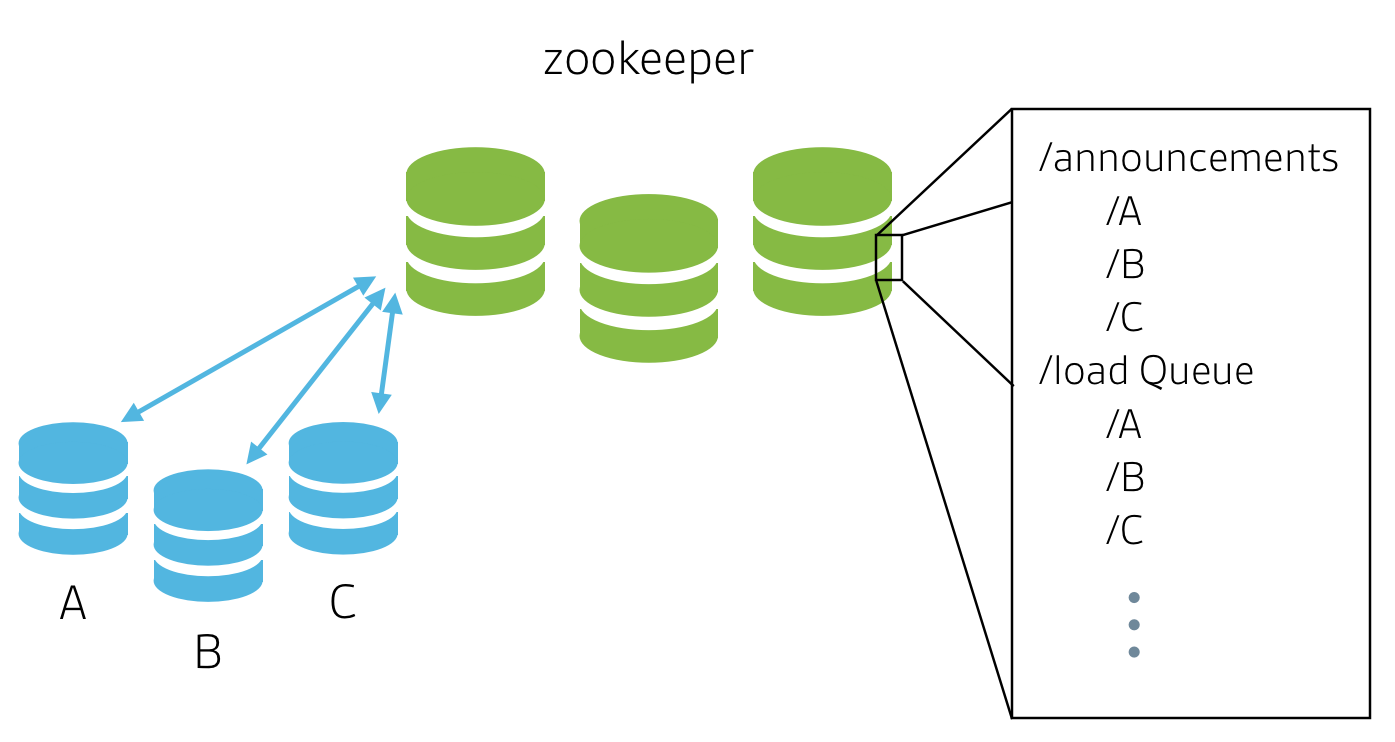
\includegraphics[width = 2.8in]{zookeeper}
\caption{Compute nodes create ephemeral znodes under specifically configured Zookeeper paths.}
\label{fig:zookeeper}
\end{figure}

To expose a segment for querying, a compute node must first possess a
local copy of the segment. Before a compute node downloads a segment
from deep storage, it first checks a local disk directory (cache) to
see if the segment already exists in local storage. If no cache
information about the segment is present, the compute node will
download metadata about the segment from Zookeeper. This metadata
includes information about where the segment is located in deep
storage and about how to decompress and process the segment. Once a
compute node completes processing a segment, the node announces (in
Zookeeper) that it is serving the segment. At this point, the segment
is queryable.

\subsubsection{Tiers}
\label{sec:tiers}
Compute nodes can be grouped in different tiers, where all nodes in a
given tier are identically configured. Different performance and
fault-tolerance parameters can be set for each tier. The purpose of
tiered nodes is to enable higher or lower priority segments to be
distributed according to their importance. For example, it is possible
to spin up a “hot” tier of compute nodes that have a high number of
cores and a large RAM capacity. The “hot” cluster can be configured to
download more frequently accessed segments. A parallel “cold” cluster
can also be created with much less powerful backing hardware. The
“cold” cluster would only contain less frequently accessed segments.

\subsection{Real-time Nodes}
\label{sec:realtime}
Real-time nodes encapsulate the functionality to ingest and query
real-time data streams. Data indexed via these nodes is immediately
available for querying. Real-time nodes are a consumer of data and
require a corresponding producer to provide the data
stream. Typically, for data durability purposes, a message bus such as
Kafka \cite{kreps2011kafka} sits between the producer and the real-time node as shown
in Figure~\ref{fig:data_reading}.

The purpose of the message bus in Figure~\ref{fig:data_reading} is to act as a buffer for
incoming events. The message bus can maintain offsets indicating the
position in an event stream that a real-time node has read up to and
real-time nodes can update these offsets periodically. The message bus also acts as backup storage for recent events.
Real-time nodes ingest data by reading events from the message bus. The time from event creation to message bus storage to
event consumption is on the order of hundreds of milliseconds.

Real-time nodes maintain an in-memory index buffer for all incoming
events. These indexes are incrementally populated as new events appear on the message bus. The indexes are also directly queryable.
Real-time nodes persist their indexes to disk either periodically or after some maximum row limit is
reached. After each persist, a real-time node updates the message bus
with the offset of the last event of the most recently persisted
index. Each persisted index is immutable. If a real-time node fails and recovers, it can simply reload
any indexes that were persisted to disk and continue reading the
message bus from the point the last offset was committed. Periodically committing offsets reduces the number of messages a real-time
node has to rescan after a failure scenario.

Real-time nodes maintain a consolidated view of the currently updating
index and of all indexes persisted to disk. This unified view allows
all indexes on a node to be queried. On a periodic basis, the nodes will
schedule a background task that searches for all persisted indexes of
a data source. The task merges these indexes together and builds a
historical segment. The nodes will upload the segment to deep storage
and provide a signal for the historical compute nodes to begin serving
the segment. The ingest, persist, merge, and handoff steps are fluid;
there is no data loss as a real-time node converts a real-time segment
to a historical one. Figure~\ref{fig:data-durability} illustrates the process.

Similar to compute nodes, real-time nodes announce segments in
Zookeeper. Unlike historical segments, real-time segments may
represent a period of time that extends into the future. For example,
a real-time node may announce it is serving a segment that contains
data for the current hour. Before the end of the hour, the real-time
node continues to collect data for the hour. Every 10 minutes (the
persist period is configurable), the node will flush and persist its
in-memory index to disk. At the end of the current hour, the real-time
node prepares to serve data for the next hour by creating a new index
and announcing a new segment for the next hour. The node does not
immediately merge and build a historical segment for the previous hour
until after some window period has passed. Having a window period
allows for straggling data points to come in and minimizes the risk of
data loss. At the end of the window period, the real-time node will
merge all persisted indexes, build a historical segment for the
previous hour, and hand the segment off to historical nodes to
serve. Once the segment is queryable on the historical nodes, the
real-time node flushes all information about the segment and
unannounces it is serving the segment.

Real-time nodes are highly scalable. If the data volume and ingestion
rates for a given data source exceed the maximum capabilities of a
single node, additional nodes can be added.  Multiple nodes can
consume events from the same stream, and every individual node only
holds a portion of the total number of events.  This creates natural
partitions across nodes. Each node announces the real-time segment it
is serving and each real-time segment has a partition number.  Data
from individual nodes will be merged at the broker level.  To our
knowledge, the largest production level real-time Druid cluster is
consuming approximately 500MB/s (150,000 events/s or 2 TB/hour of raw data).

\begin{figure}
\centering
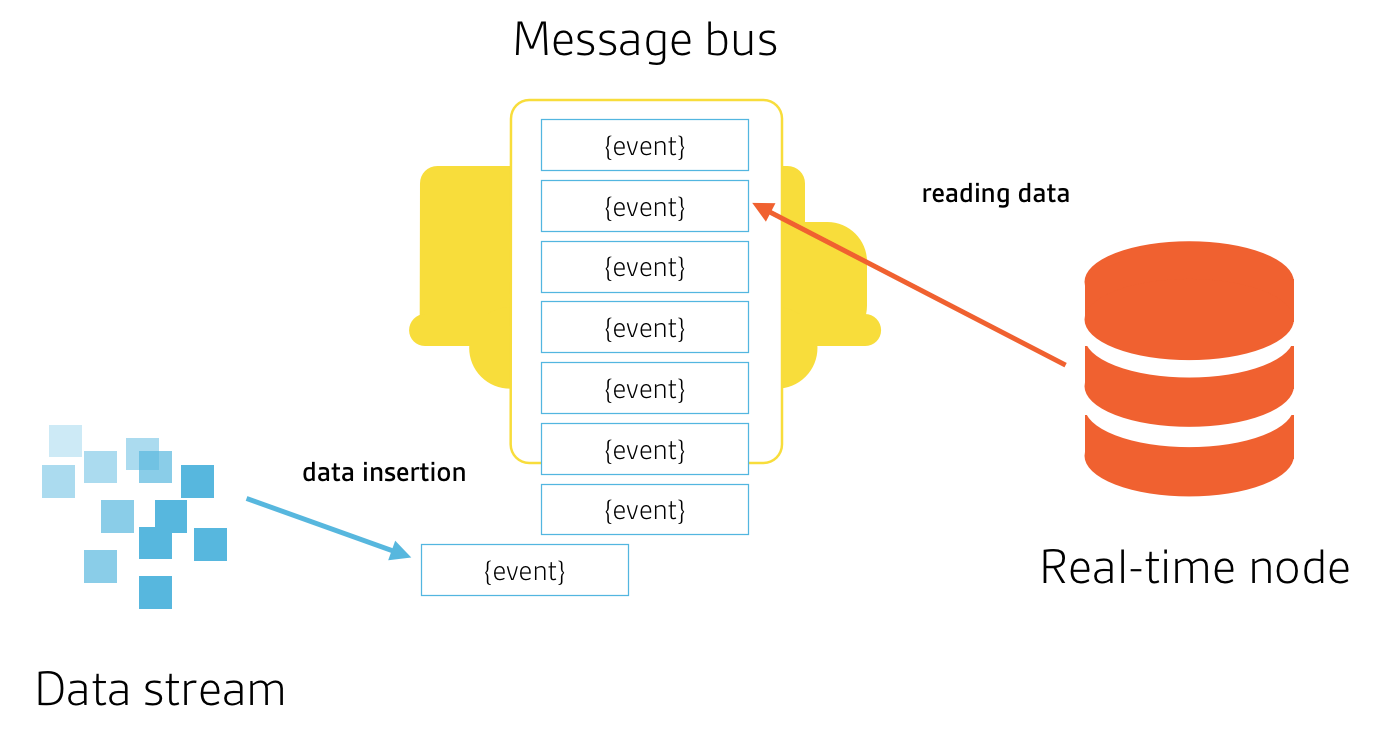
\includegraphics[width = 2.8in]{data_reading}
\caption{Real-time data ingestion.}
\label{fig:data_reading}
\end{figure}

\begin{figure}
\centering
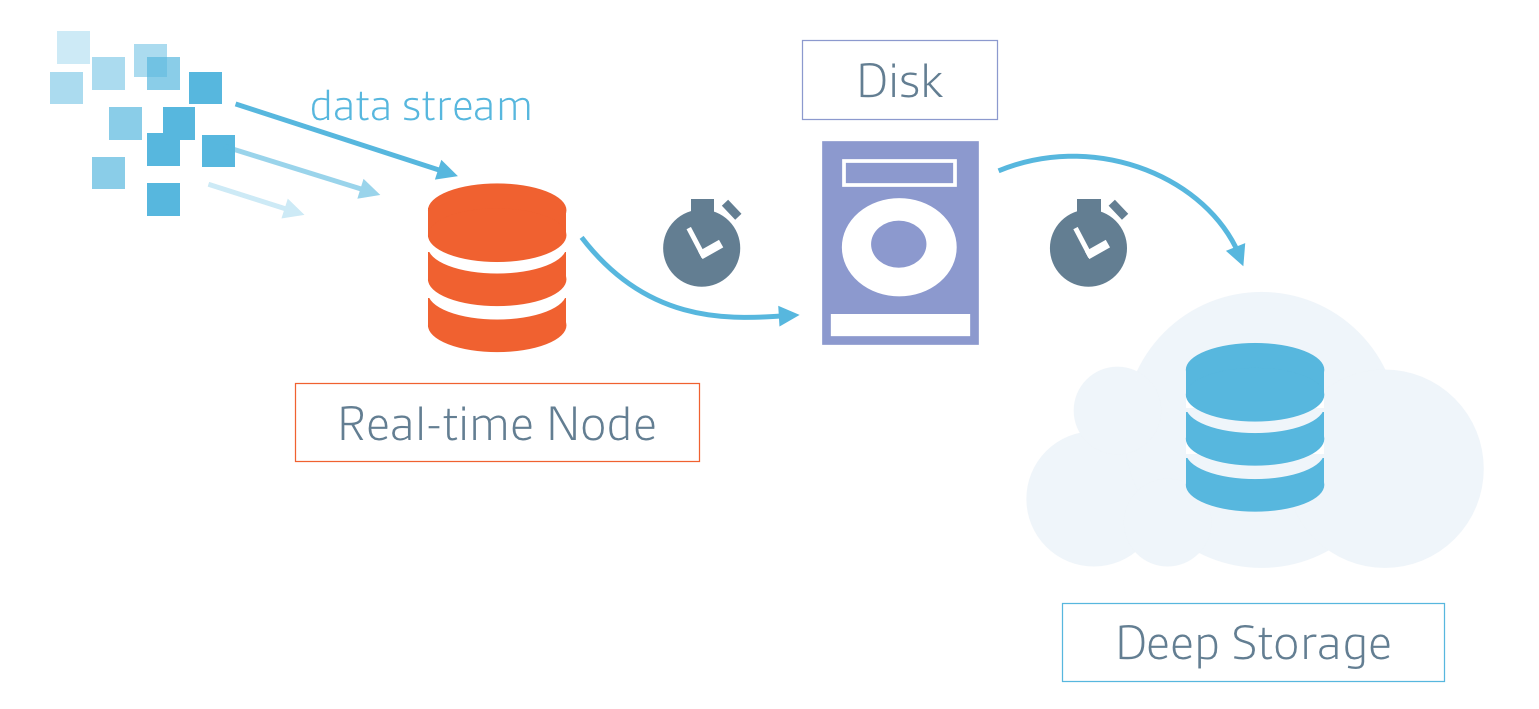
\includegraphics[width = 2.8in]{druid_realtime_flow}
\caption{Real-time data durability}
\label{fig:data-durability}
\end{figure}

\subsection{Broker Nodes}
Broker nodes act as query routers to other queryable nodes such as
compute and real-time nodes. Broker nodes understand the metadata
published in Zookeeper about what segments exist and on what nodes the
segments are stored. Broker nodes route incoming queries such that the queries hit
the right storage nodes. Broker nodes also merge partial results from
storage nodes before returning a final consolidated result to the
caller.  Additionally, brokers provide an extra level of data
durability as they maintain a cache of recent results. In the event
that multiple storage nodes fail and all copies of a segment are
somehow lost, it is still possible that segment results can still be
returned if that information exists in the cache.

\subsubsection{Timeline}
To determine the correct nodes to forward queries to, brokers
first build a view of the world from information in Zookeeper. Recall
that Druid uses Zookeeper to maintain information about all compute
and real-time nodes in a cluster and the segments those nodes are
serving. For every data source in Zookeeper, the broker node builds a
timeline of segments for the data source and the nodes that serve them. A timeline
consists of segments and represents which segments contain data for
what ranges of time. Druid may have multiple segments where the data
source and interval are the same but versions differ. The timeline
view will always surface segments with the most recent version
identifier for a time range. If two segments intervals overlap, the segment with the more recent
version always has precedence. When queries are received for a specific
data source and interval, the broker node performs a lookup on the
timeline associated with the query data source for the query interval
and retrieves the segments that contain data for the query. The broker
node maps these segments to the storage nodes that serve them and
forwards the query down to the respective nodes.


\subsubsection{Caching}
\label{sec:caching}
Broker nodes employ a distributed cache with a LRU \cite{o1993lru,
kim2001lrfu} cache invalidation strategy. The broker cache stores
per segment results. The cache can be local to each broker node or
shared across multiple nodes using an external distributed cache
such as memcached \cite{fitzpatrick2004distributed}. Recall that each time a broker node receives a
query, it first maps the query to a set of segments. A subset of
these segment results may already exist in the cache and the results
can be directly pulled from the cache. For any segment results that
do not exist in the cache, the broker node will forward the query
to the compute nodes. Once the compute nodes return their results,
the broker will store those results in the cache. Real-time segments
are never cached and hence requests for real-time data will always
be forwarded to real-time nodes. Real-time data is perpetually
changing and caching the results would be unreliable.


\subsection{Coordination (Master) Nodes}
The Druid coordination or master nodes are primarily in charge of
segment management and distribution. The Druid master is responsible
for loading new segments, dropping outdated segments, managing segment
replication, and balancing segment load. Druid uses a multi-version
concurrency control swapping protocol for managing segments in order
to maintain stable views.

The Druid master runs periodically to determine the current state of
the cluster. It makes decisions by comparing the expected state of the
cluster with the actual state of the cluster at the time of the
run. As with all Druid nodes, the Druid master maintains a connection
to Zookeeper for current cluster information. The master also
maintains a connection to a MySQL database that contains additional
operational parameters and configurations. One of the key pieces of
information located in the MySQL database is a segment table that
contains a list of historical segments that should be served. This
table can be updated by any service that creates historical
segments. The MySQL database also contains a rule table that governs
how segments are created, destroyed, and replicated in the cluster.

The master does not directly communicate with a compute node when
assigning it work; instead the master creates an ephemeral znode in
Zookeeper containing information about what the compute node should
do. The compute node maintains a similar connection to Zookeeper to
monitor for new work.

\subsubsection{Rules}
Rules govern how historical segments are loaded and dropped from the cluster. 
Rules indicate how segments should be assigned to
different compute node tiers and how many replicates of a segment
should exist in each tier. Rules may also indicate when segments
should be dropped entirely from the cluster. Rules are usually set for a period of time. 
For example, a user may use rules to load the most recent one month's worth of segments into a "hot" cluster, 
the most recent one year's worth of segments into a "cold" cluster, and drop any segments that are older.

The master loads a set of
rules from a rule table in the MySQL database. Rules may be specific
to a certain data source and/or a default set of rules may be
configured. The master will cycle through all available segments and
match each segment with the first rule that applies to it.

\subsubsection{Load Balancing}
In a typical production environment, queries often hit dozens or even
hundreds of data segments. Since each compute node has limited
resources, historical segments must be distributed among the cluster
to ensure that the cluster load is not too imbalanced. Determining
optimal load distribution requires some knowledge about query patterns
and speeds. Typically, queries cover recent data spanning contiguous
time intervals for a single data source.  On average, queries that
access smaller segments are faster.

These query patterns suggest replicating recent historical segments at
a higher rate, spreading out large segments that are close in time to
different compute nodes, and co-locating segments from different data
sources.  To optimally distribute and balance segments among the
cluster, we developed a cost-based optimization procedure that takes
into account the segment data source, recency, and size. The exact
details of the algorithm are beyond the scope of this paper and may be discussed in future literature.

\section{Query API}
\label{sec:query-api}
Druid has its own query language and accepts queries as POST requests. All queryable
Druid nodes share the same query API.

The body of the POST request is
a JSON object containing key-value pairs specifying various query
parameters. A typical query will contain the data source name, the
granularity of the result data, time range of interest, the
type of request, and the metrics to aggregate over. The result will also be a JSON object
containing the aggregated metrics over the time period.

Most query types will also support a filter set. A filter set is a Boolean expression of dimension name and value
pairs. Any number and combination of dimensions and values may be specified.
When a filter set is provided, only the subset of the data that pertains to the filter set will be scanned.
The ability to handle complex nested filter sets is what enables Druid 
to drill into data at any depth.

The exact query syntax depends on the query type and the information requested.
A sample time series query is shown below:
\begin{verbatim}
{
  "queryType"     : "timeseries",
  "dataSource"    : "sample_data",
  "intervals"     : "2013-01-01/2013-01-02",
  "filter"        : {
    "type"        : "selector",
    "dimension"   : "poets",
    "value"       : "Ke$ha"
  },
  "granularity"   : "day",
  "aggregations"  : [
    {
      "type"      : "count",
      "fieldName" : "row",
      "name"      : "row"
    }
  ]
}
\end{verbatim}

It is beyond the scope of this paper to fully describe the query API.
We are also in the process of extending the Druid API to understand SQL.

\section{Storage}
\label{sec:storage}
Druid is a column-oriented data store. When considering aggregates
over a large number of events, the advantages storing data as columns
rather than rows are well documented \cite{cattell2011scalable}. Column storage allows for
more efficient CPU usage as only what is needed is actually loaded and
scanned. In a row oriented data store, all columns associated with a
row must be scanned as part of an aggregation. The additional scan
time can introduce performance degradations as high as 250\% \cite{bear2012vertica}.

\subsection{Column Types}
Druid has multiple column types to represent the various column value
formats. Depending on the column type, different compression methods
are used to reduce the cost of storing a column in memory and on
disk. In the example given in Table~\ref{tab:sample_data}, the
publisher, advertiser, gender, and country columns only contain
strings. String columns can be dictionary encoded. Dictionary encoding
is a common method to compress data and has been used in other data
stores such as PowerDrill \cite{hall2012processing}. In the example in
Table~\ref{tab:sample_data}, we can map each publisher to an unique
integer identifier.
\begin{verbatim}
bieberfever.com   -> 0
ultratrimfast.com -> 1
\end{verbatim}
This mapping allows us to represent the publisher column as an integer
array where the array indices correspond to the rows of the original
data set. For the publisher column, we can represent the unique
publishers as follows:
\begin{verbatim}
[0, 0, 1, 1]
\end{verbatim}

The resulting integer array lends itself very well to
compression methods. Generic compression algorithms on top of encodings are
extremely common in column-stores. Druid uses the LZF \cite{liblzf2013} compression
algorithm.

Similar compression methods can be applied to numeric
columns. For example, the clicks and revenue columns in
Table~\ref{tab:sample_data} can also be expressed as individual
arrays.
\begin{verbatim}
Clicks  -> [25, 42, 17, 170]
Revenue -> [15.70, 29.18, 17.31, 34.01]
\end{verbatim}
In this case we compress the raw values as opposed to their dictionary
representations.

\subsection{Filters}
To support arbitrary filter sets, Druid creates additional lookup
indices for string columns. These lookup indices are compressed and
Druid operates over the indices in their compressed form. Filters can
be expressed as Boolean equations of multiple lookup indices. Boolean
operations of indices in their compressed form is both performance and
space efficient.

Let us consider the publisher column in
Table~\ref{tab:sample_data}. For each unique publisher in
Table~\ref{tab:sample_data}, we can form some representation
indicating which table rows a particular publisher is seen. We can
store this information in a binary array where the array indices
represent our rows. If a particular publisher is seen in a certain
row, that array index is marked as \texttt{1}. For example:
\begin{verbatim}
bieberfever.com   -> rows [0, 1] -> [1][1][0][0]
ultratrimfast.com -> rows [2, 3] -> [0][0][1][1]
\end{verbatim}

\texttt{\href{http://bieberfever.com}{bieberfever.com}} is seen in rows \texttt{0} and \texttt{1}. This mapping of column values
to row indices forms an inverted index \cite{tomasic1993performance}. To know which
rows contain {\ttfamily bieberfever.com} or {\ttfamily ultratrimfast.com}, we can \texttt{OR} together
the two arrays.
\begin{verbatim}
[0][1][0][1] OR [1][0][1][0] = [1][1][1][1]
\end{verbatim}

\begin{figure}
\centering
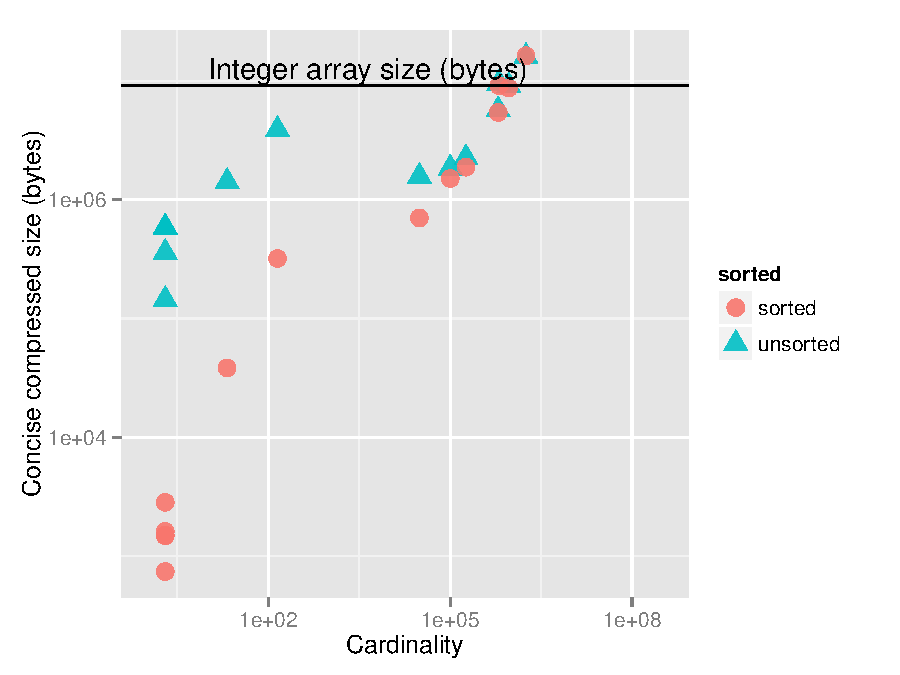
\includegraphics[width = 3in]{concise_plot}
\caption{Integer array size versus Concise set size.}
\label{fig:concise_plot}
\end{figure}

This approach of performing Boolean operations on large bitmap sets is
commonly used in search engines. Bitmap compression algorithms are a
well-defined area of research and often utilize run-length
encoding. Popular algorithms include Byte-aligned Bitmap Code \cite{antoshenkov1995byte},
Word-Aligned Hybrid (WAH) code \cite{wu2006optimizing}, and Partitioned Word-Aligned
Hybrid (PWAH) compression \cite{van2011memory}. Druid opted to use the Concise
algorithm \cite{colantonio2010concise} as it can outperform WAH by reducing the size of the
compressed bitmaps by up to 50\%.  Figure~\ref{fig:concise_plot} illustrates the number of
bytes using Concise compression versus using an integer array. The
results were generated on a cc2.8xlarge system with a single thread,
2G heap, 512m young gen, and a forced GC between each run. The data
set is a single day’s worth of data collected from the Twitter garden
hose \cite{twitter2013} data stream. The data set contains 2,272,295 rows and 12
dimensions of varying cardinality. As an additional comparison, we
also resorted the data set rows to maximize compression.

In the unsorted case, the total Concise size was 
53,451,144 bytes and the total integer array size was 127,248,520 bytes. Overall,
Concise compressed sets are about 42\% smaller than integer arrays.
In the sorted case, the total Concise compressed size was 43,832,884
bytes and the total integer array size was 127,248,520 bytes.  What is
interesting to note is that after sorting, global compression only
increased minimally. The total Concise set size to total integer array
size is 34\%. It is also interesting to note that as the cardinality
of a dimension approaches the total number of rows in a data set,
integer arrays require less space than Concise sets and become a better alternative.

\subsection{Storage Engine}
Druid’s persistence components allows for different storage engines to
be plugged in, similar to Dynamo \cite{decandia2007dynamo}. These storage engines may store
data in in-memory structures such as the JVM heap or in memory-mapped
structures. The ability to swap storage engines allows for Druid to be
configured depending on a particular application’s specifications. An
in-memory storage engine may be operationally more expensive than a
memory-mapped storage engine but could be a better alternative if
performance is critical. At Metamarkets, we commonly use a
memory-mapped storage engine.

\section{Robustness}
\label{sec:robustness}
To achieve high system availability and data durability, Druid employs
several fault recovery techniques. Druid has no single point of
failure.

\subsection{Replication}
Druid replicates historical segments on multiple hosts. The number of
replicates in each tier of the historical compute cluster is fully
configurable. Setups that require high levels of fault tolerance can
be configured to have a high number of replicates. Replicates are
assigned to compute nodes by coordination nodes using the same load
distribution algorithm discussed in Section~\ref{sec:caching}. Broker nodes forward queries to the first node they find that contain a segment required for the query.

Real-time segments follow a different replication model as real-time
segments are mutable. Multiple real-time nodes can read from the same message
bus and event stream if each node maintains a unique offset and consumer id, hence creating multiple copies
of a real-time segment. This is conceptually different than multiple
nodes reading from the same event stream and sharing the same offset and consumer id, doing so would create
multiple segment partitions. If a real-time node fails and recovers, it can
reload any indexes that were persisted to disk and read from the
message bus from the point it last committed an offset.

\subsection{Failure Detection}
If a compute node completely fails and becomes unavailable, the
ephemeral Zookeeper znodes it created are deleted. The master node
will notice that certain segments are insufficiently replicated or
missing altogether. Additional replicates will be created and
redistributed throughout the cluster.

We are moving towards building out infrastructure to support
programmatic creation of real-time nodes. In the near future, the
master node or a similar service will notice if real-time segments are insufficiently
replicated and automatically create additional real-time nodes as
redundant backups.

Coordination and broker nodes always have redundant backup nodes in the event
the primary fails. The backup nodes are usually idle until Zookeeper changes alert
them to assume the responsibilities of their primary counterparts.

\subsection{Adding and Removing Nodes}
Starting and removing Druid nodes is done by starting and stopping Java processes. There is minimal
operational overhead with adding nodes in batches. Scaling down the
cluster is usually done one node at a time with some time lapse
between shutdowns. This allows the master to have ample time to
redistribute load and create additional replicates. Shutting down
nodes in batches is not recommended as it may destroy all
copies of a segment, which would lead to data loss.

\section{Performance Benchmarks}
\label{sec:benchmarks}
\begin{figure}
\centering
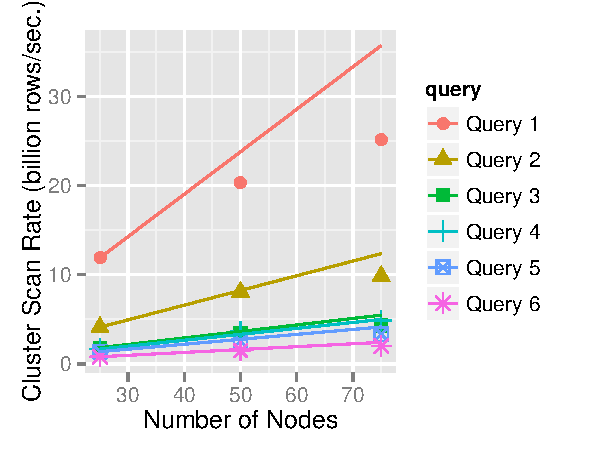
\includegraphics[width = 2.8in]{cluster_scan_rate}
\caption{Druid cluster scan rate with lines indicating linear scaling
  from 25 nodes.}
\label{fig:cluster_scan_rate}
\end{figure}
To benchmark Druid performance, we created a large test cluster with
6TB of uncompressed data, representing tens of billions of fact
rows. The data set contained more than a dozen dimensions, with
cardinalities ranging from the double digits to tens of millions. We computed
four metrics for each row (counts, sums, and averages). The data was
sharded first on timestamp then on dimension values, creating
thousands of shards roughly 8 million fact rows apiece.

The cluster used in the benchmark consisted of 100 historical compute
nodes, each with 16 cores, 60GB of RAM, 10 GigE Ethernet, and 1TB of
disk space. Collectively, the cluster comprised of 1600 cores, 6TB or
RAM, sufficiently fast Ethernet and more than enough disk space.

SQL statements are included in Table~\ref{tab:sql_queries} to describe the
purpose of each of the queries. Please note:
\begin{itemize}
\item The timestamp range of the queries encompassed all data.
\item Each machine was a 16-core machine with 60GB RAM and 1TB of local
  disk. The machine was configured to only use 15 threads for
  processing queries.
\item A memory-mapped storage engine was used (the machine was configured to memory map the data
  instead of loading it into the Java heap.)
\end{itemize}

\begin{figure}
\centering
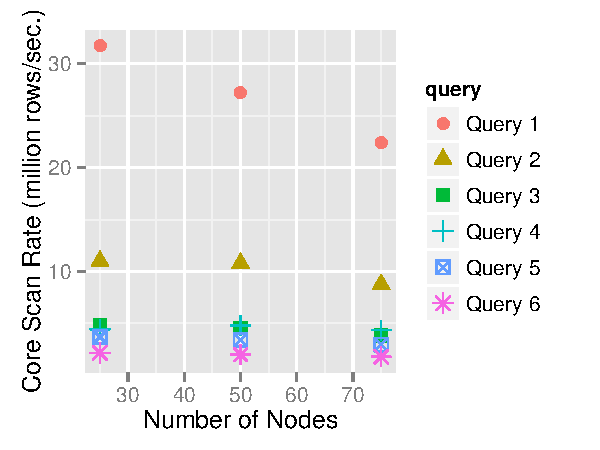
\includegraphics[width = 2.8in]{core_scan_rate}
\caption{Druid core scan rate.}
\label{fig:core_scan_rate}
\end{figure}

\begin{table*}
  \centering
  \caption{Druid Queries}
  \label{tab:sql_queries}
  \begin{tabular}{| l | p{15cm} |}
    \hline
    \textbf{Query \#} & \textbf{Query} \\ \hline
    1 & \texttt{SELECT count(*) FROM \_table\_ WHERE timestamp $\geq$ ? AND timestamp < ?} \\ \hline
    2 & \texttt{SELECT count(*), sum(metric1) FROM \_table\_ WHERE timestamp $\geq$ ? AND timestamp < ?} \\ \hline
    3 & \texttt{SELECT count(*), sum(metric1), sum(metric2), sum(metric3), sum(metric4) FROM \_table\_ WHERE timestamp $\geq$ ? AND timestamp < ?} \\ \hline
    4 & \texttt{SELECT high\_card\_dimension, count(*) AS cnt FROM \_table\_ WHERE timestamp $\geq$ ? AND timestamp < ? GROUP BY high\_card\_dimension ORDER BY cnt limit 100} \\ \hline
    5 & \texttt{SELECT high\_card\_dimension, count(*) AS cnt, sum(metric1) FROM \_table\_ WHERE timestamp $\geq$ ? AND timestamp < ? GROUP BY high\_card\_dimension ORDER BY cnt limit 100} \\ \hline
    6 & \texttt{SELECT high\_card\_dimension, count(*) AS cnt, sum(metric1), sum(metric2), sum(metric3), sum(metric4) FROM \_table\_ WHERE timestamp $\geq$ ? AND timestamp < ? GROUP BY high\_card\_dimension ORDER BY cnt limit 100} \\ \hline
  \end{tabular}
\end{table*}

Figure~\ref{fig:cluster_scan_rate} shows the cluster scan rate and
Figure~\ref{fig:core_scan_rate} shows the core scan rate.  In
Figure~\ref{fig:cluster_scan_rate} we also include projected linear
scaling based on the results of the 25 core cluster.  In particular,
we observe diminishing marginal returns to performance in the size of
the cluster.  Under linear scaling, SQL query 1 would have achieved a
speed of 37 billion rows per second on our 75 node cluster.  In fact,
the speed was 26 billion rows per second.  However, queries 2-6 maintain
a near-linear speedup up to 50 nodes: the core scan rates in
Figure~\ref{fig:core_scan_rate} remain nearly constant.
The increase in speed of a parallel
computing system is often limited by the time needed for the
sequential operations of the system, in accordance with Amdahl's law
\cite{amdahl1967validity}.

The first query listed in Table~\ref{tab:sql_queries} is a simple
count, achieving scan rates of 33M rows/second/core. We believe
the 75 node cluster was actually overprovisioned for the test
dataset, explaining the modest improvement over the 50 node cluster.
Druid's concurrency model is based on shards: one thread will scan one
shard. If the number of segments on a compute node modulo the number
of cores is small (e.g. 17 segments and 15 cores), then many of the
cores will be idle during the last round of the computation.

When we include more aggregations we see performance degrade.  This is
because of the column-oriented storage format Druid employs.  For the
\texttt{count(*)} queries, Druid only has to check the timestamp column to satisfy
the ``where'' clause.  As we add metrics, it has to also load those metric
values and scan over them, increasing the amount of memory scanned.

\section{Related Work}
\label{sec:related}
Cattell \cite{cattell2011scalable} maintains a great summary about existing Scalable SQL and
NoSQL data stores. Druid
feature-wise sits somewhere between Google’s Dremel \cite{melnik2010dremel} and PowerDrill
\cite{hall2012processing}. Druid has most of the features implemented in Dremel (Dremel
handles arbitrary nested data structures while Druid only allows for a
single level of array-based nesting) and many of the interesting
compression algorithms mentioned in PowerDrill.

Although Druid builds on many of the same principles as other
distributed columnar data stores \cite{fink2012distributed}, most existing data
stores are designed to be key-value stores \cite{lerner2010redis}, or
document/extensible record stores \cite{stonebraker2005c}. Such data stores are great
solutions for traditional data warehouse needs and general
back-office/reporting usage. Typically, analysts will query these data
stores and build reports from the results. In-memory databases such as
SAP’s HANA \cite{farber2012sap} and VoltDB \cite{voltdb2010voltdb} are examples of other data stores that
are highly suited for traditional data warehousing needs. Druid is a
front-office system designed such that user-facing dashboards can be
built on top of it. Similar to \cite{paraccel2013}, Druid has analytical features
built in. The main features Druid offers over traditional data
warehousing solutions are real-time data ingestion, interactive
queries and interactive query latencies. In terms of real-time
ingestion and processing of data, Trident/Storm \cite{marz2013storm} and Streaming
Spark \cite{zaharia2012discretized} are other popular real-time computation systems, although
they lack the data storage capabilities of Druid. Spark/Shark \cite{engle2012shark} are
also doing similar work in the area of fast data analysis on large
scale data sets. Cloudera Impala \cite{cloudera2013} is another system focused on
optimizing querying performance, but more so in Hadoop environments.

Druid leverages a unique combination of algorithms in its
architecture. Although we believe no other data store has the same set
of functionality as Druid, some of Druid’s optimization techniques such as using
inverted indices to perform fast filters are also used in other data
stores \cite{macnicol2004sybase}.

\section{Conclusions}
\label{sec:conclusions}
In this paper, we presented Druid, a distributed, column-oriented,
real-time analytical data store. Druid is a highly customizable
solution that is optimized for fast query latencies. Druid ingests
data in real-time and is fault-tolerant. We discussed the performance
of Druid on billion row data sets. We summarized key Druid architecture
aspects such as the storage format, query language and general
execution. In the future, we plan to cover more in depth the different
algorithms we’ve developed for Druid and how other systems may plug
into Druid to achieve powerful use cases.

\balance

\section{Acknowledgements}
\label{sec:acknowledgements}
We want to thank Steve Harris for his feedback on improving this paper, Adam Smith for giving us the chance to write this paper, and Katherine Chu for
helping to create all the images in this paper. Druid could not have been built without the help of many great
engineers at Metamarkets and in the community. We want to thank Danny Yuan, Jae Hyeon Bae, Paul Baclace, Dave
Nielsen, and Dhruv Parthasarathy for their
contributions to Druid.

% The following two commands are all you need in the
% initial runs of your .tex file to
% produce the bibliography for the citations in your paper.
\bibliographystyle{abbrv}
\bibliography{druid}  % druid.bib is the name of the Bibliography in this case
% You must have a proper ".bib" file
%  and remember to run:
% latex bibtex latex latex
% to resolve all references

%Generated by bibtex from your ~.bib file.  Run latex,
%then bibtex, then latex twice (to resolve references).

%APPENDIX is optional.
% ****************** APPENDIX **************************************
% Example of an appendix; typically would start on a new page
%pagebreak

\end{document}
